\documentclass{amia}
\usepackage[utf8x]{inputenc}
\usepackage{graphicx}
\usepackage{listings}
\usepackage[labelfont=bf]{caption}
\usepackage[superscript,nomove]{cite}
\usepackage{color}
\usepackage{caption}
\usepackage{todonotes}
\usepackage{url}
\newcommand{\remPierre}[1]{\todo[color=green]{[PZ]{\scriptsize #1\par}}}
\newcommand{\remXavier}[1]{\todo[color=yellow]{[XT]{\scriptsize #1\par}}}
\newcommand{\remNico}[1]{\todo[color=orange]{[NP]{\scriptsize #1\par}}}
\newcommand{\remTom}[1]{\todo[color=red]{[TP]{\scriptsize #1\par}}}


\newcommand\YAMLcolonstyle{\color{red}\mdseries}
\newcommand\YAMLkeystyle{\color{black}\bfseries}
\newcommand\YAMLvaluestyle{\color{blue}\mdseries}

\makeatletter

% here is a macro expanding to the name of the language
% (handy if you decide to change it further down the road)
\newcommand\language@yaml{yaml}

\expandafter\expandafter\expandafter\lstdefinelanguage
\expandafter{\language@yaml}
{
  keywords={true,false,null,y,n},
  keywordstyle=\color{darkgray}\bfseries,
  basicstyle=\YAMLkeystyle,                                 % assuming a key comes first
  sensitive=false,
  comment=[l]{\#},
  morecomment=[s]{/*}{*/},
  commentstyle=\color{blue}\ttfamily,
  stringstyle=\YAMLvaluestyle\ttfamily,
  moredelim=[l][\color{orange}]{\&},
  moredelim=[l][\color{magenta}]{*},
  moredelim=**[il][\YAMLcolonstyle{:}\YAMLvaluestyle]{:},   % switch to value style at :
  morestring=[b]',
  morestring=[b]",
  literate =    {---}{{\ProcessThreeDashes}}3
                {>}{{\textcolor{red}\textgreater}}1     
                {|}{{\textcolor{red}\textbar}}1 
                {\ -\ }{{\mdseries\ -\ }}3,
}

% switch to key style at EOL
\lst@AddToHook{EveryLine}{\ifx\lst@language\language@yaml\YAMLkeystyle\fi}
\makeatother

\newcommand\ProcessThreeDashes{\llap{\color{cyan}\mdseries-{-}-}}
\begin{document}


\title{i2b2 implemented over SMART-on-FHIR} 
\author{Nicolas Paris, MSc.$^{1,2,3}$, Michael Mendis$^{4}$, Shawn Murphy, MD, Ph.D$^{4}$, Xavier Tannier, Ph.D$^{3,5}$, Pierre Zweigenbaum, Ph.D$^{2}$
}

\institutes{
    $^1$WIND-DSI, AP-HP, Paris, France; $^2$LIMSI, CNRS, Université Paris-Saclay, Orsay, France; $^3$INSERM, UMR\_S 1142, LIMICS, Paris, France; $^4$Partners Healthcare In., Boston, MA, USA; $^5$Sorbonne Universités, UPMC Univ
Paris 06.
    }

\maketitle

\noindent{\bf Abstract}

\textit{Integrating Biology and the Bedside (i2b2) is the de-facto open-source medical tool for cohort discovery. Fast Healthcare Interoperability Resources (FHIR) is a new standard for exchanging health care information electronically. Substitutable Modular third-party Applications (SMART) defines the SMART-on-FHIR specification on how applications shall interface with Electronic Health Records (EHR) through FHIR. Related work made it possible to produce FHIR from an i2b2 instance or i2b2 to store FHIR datasets. In this paper, we extend i2b2 to search remotely into one or multiple SMART-on-FHIR Application Programming Interfaces (APIs). This enables the federation of queries, security, terminology mapping, and also bridges the gap between i2b2 and modern big-data technologies.}

\section*{Introduction}
% A short background and objective(s) of the study
%\remPierre{L'article actuellement fait trop ingénierie à mon avis. Il faudrait dans l'introduction commencer par établier les problèmes à résoudre (quelles sont les limitations des EHR actuels ?), puis indiquer des solutions envisagées ou testées dans les travaux antérieurs (...) et finir sur celle que tu proposes. L'évaluation devrait montrer dans quelle mesure ton travail résout les problèmes notés au départ.}
%\remNico{j'ai fait les modifs suivantes dans le déroulé(je rajouterai une couche de vernis, si tant est que c'est mieux qu'avant): Objectif(learning health system);Solution actuelle(i2b2);problemes posés;solutions(FHIR);RelatedWork;Solution proposée.}
%\remPierre{Bien ; il faudrait que les paragraphes annoncent explicitement qu'ils présentent une solution personnelle, ou un problème à résoudre, etc. Actuellement les deux premiers paragraphes donnent bien le contexte, le troisième donne bien les problèmes restant à résoudre. On attend aux paragraphes suivants une annonce des solutions proposées à ces problèmes.}
%\remNico{l'enchainement est il plus clair désormais ?}
Learning Health Systems aim to maximize the potential of large-scale, harmonized data from variable, quickly-developing digital sources such as Electronic Health Records (EHRs), which are emerging as powerful tools to facilitate discoveries that can improve health. Data heterogeneity is one of the critical problems in analyzing, reusing, sharing or linking datasets. With the development of platforms enabling the linking and federation of phenome, genome and exposome data across sites in US\cite{Gottesman_2013,McMurry_2013} Europe\cite{DeMoor_2015,Delaney_2015} or at international scale\cite{Hripcsak_2015} a key challenge is to define harmonized access to heterogeneous EHR-based data.

i2b2 is the de-facto open-source medical tool for cohort discovery and allows healthcare practitioners to easily subset patient data to address research questions. I2b2 has been described as being used by more than 200 hospitals\cite{pmid22081225} over the world, and the recent migration of i2b2 to GitHub has facilitated development work. The tool is flexible, supporting its own star schema and ontology model as well as exploiting alternative information models such as PCORnet\cite{Klann_2016} and the OMOP common data model\cite{i2b2-omop} without requiring changes to the underlying data. Many initiatives have extended the primary goal of cohort discovery, providing functionality to carry out statistical analysis in place, as well as federated queries over multiple centers, and even genomic analytics.\cite{Scheufele__2014,i2b2-transmart}. Three well-known tools that extend the i2b2 functionality in this way include SHRINE, INSITE, and TRINETX \cite{shrine,insite,trinetx}.   
% * <tpollard@mit.edu> 13:21:40 28 Sep 2017 UTC-0400:
% is there a citation for "200 hospitals over the world"?
% ^ <niparisco@gmail.com> 21:22:34 28 Sep 2017 UTC+0200:
% done
% * <tpollard@mit.edu> 13:20:07 28 Sep 2017 UTC-0400:
% "on github" -> "to GitHub"
% * <tpollard@mit.edu> 13:19:02 28 Sep 2017 UTC-0400:
% I'm not clear exactly what you mean by "on place". Perhaps something like: Many initiatives have extended this primary goal, but providing functionality to carry out statistical analysis with federated queries across multiple centers"
% ^ <niparisco@gmail.com> 21:22:46 28 Sep 2017 UTC+0200:
% done

i2b2 and derived solutions do have room for improvement. For example, in terms of \textit{data variety}, federation tools such as SHRINE, INSITE, and TRINETX are inconsistent in terms of their terminology mapping processes.\cite{McMurry_2013} Where mapping details are provided \cite{ehr4crlesson}, they are time consuming and software specific\cite{Wynden__2010}. In terms of \textit{freshness of the data}, Extract Transform Load processes (ETL) feeding traditional relational databases supported by the i2b2 tools (e.g. postgreSQL, Oracle, MSSQL) are resource consuming, taking considerable amounts of time, maintenance, and disk-space. Though ETL procedures are still feasible these days, the emergence of high-throughput healthcare data and the "Internet of Things" demands the development of new approaches that allow data to be queried in place (i.e. directly within EHRs) or in optimized, dedicated places such RDF triple stores. The time delta due to data migrations and transformations poses problems of \textit{data veracity} because the source data is susceptible to be modified in the interval, and multiple transformation are error prone.  In terms of \textit{data volume}, data producers of interest for patient care such omics, exposomics, imaging or free text notes are challenging to store and also to analyze. In order for the data to be analyzed properly and efficiently, specialized and dedicated technology are required. While there have been several engineering attempts to create i2b2 based data-warehouses solutions that work with technologies other than traditional relational databases\cite{Wang2014}, the cost to create such interfaces is high. The i2b2 star schema model is highly optimized for fast retrieving lists of patients matching criteria, but it is not intended for statistical analytics or data exploration\cite{pmid27577447}. Although there are some bridges with other common data-models such as OMOP, the architecture is still based on RDBMS\cite{Klann_2016}. The emergence of new technology is faster than i2b2's ability to exploit them. In terms of \textit{software accessibility}, for example, physicians spend time switching between applications, writing their login and password credentials again \& again. Providing these users with the ``one login/multiple application'' paradigm would optimize the time spent on the computer and thus improve patient care.  
% * <tpollard@mit.edu> 14:27:26 28 Sep 2017 UTC-0400:
% what is it about the "Internet of Things" that makes ETL less feasible? e.g. multiple data sources?
% ^ <niparisco@gmail.com> 21:24:03 28 Sep 2017 UTC+0200:
% yes web3 needs triple store or graph database

% * <tpollard@mit.edu> 14:16:25 28 Sep 2017 UTC-0400:
% It isn't completely clear from this sentence ("Providing these users with the "one login/multiple application" paradigm..") why having a single login would mean stronger passwords, so perhaps this could be better explained.
% ^ <niparisco@gmail.com> 21:27:44 28 Sep 2017 UTC+0200:
% right, I try to explain better
% ^ <niparisco@gmail.com> 21:28:42 28 Sep 2017 UTC+0200:
% removed

% * <tpollard@mit.edu> 13:32:02 28 Sep 2017 UTC-0400:
% It is not clear to me which list the "each federation tool listed below" comment is referring to. i.e. where is the list of federation tools?
% * <tpollard@mit.edu> 13:29:55 28 Sep 2017 UTC-0400:
% "ingeniering" -> "ingenious" or "engineering" perhaps?
% ^ <niparisco@gmail.com> 21:26:51 28 Sep 2017 UTC+0200:
% yes engineering thx
The solution explored in this work is to bring the latest accomplishments of the Health Level Seven (HL7) Fast Healthcare Interoperability Resources (FHIR) community to i2b2. In particular, to bring the flexibility, the extensibility, the standardization, and the interoperability efforts to i2b2. In the domain of patient care, several large-scale efforts have been underway for over a decade with the goal of specifying both the structure and the semantics of patient clinical information in a manner that enables computable semantic interoperability between diverse systems. Although there is no consensus in the medical informatics community regarding a standard patient information model, FHIR specifications are gaining interest and show promise to mitigate the classic site-specific data mapping problem. FHIR is built on lessons\cite{Rosenbloom_2017} from previous standards, including the Reference Information Model (RIM) which became an ISO standard in 2003, and the Clinical Document Architecture designed to express a single clinical document as a message using HL7 version 3 RIM classes. FHIR specifies a RESTful API to access resources. Several initiatives facilitate the adoption of FHIR, including the Argonaut project\cite{argo} and the Clinical Information Modeling Initiative (CIMI)\cite{cimi}. 
SMART-on-FHIR\cite{smarton} is an open, standards based technology platform that enables innovators to create apps that seamlessly and securely run across the healthcare system. Using EHRs or data warehouse that supports the SMART standard, patients, doctors, and healthcare practitioners can draw on this library of applications to improve clinical care, research, and public health. SMART success improve the user experience exactly the same major Internet provide access to many application with a single authentication, and proposes now more than 50 applications, able to consume one unique FHIR-API.
% * <tpollard@mit.edu> 14:36:24 28 Sep 2017 UTC-0400:
% I am unclear how the "SMART Health IT ..." sentence relates to the rest of the paragraph. Is "SMART Health IT " the solution that you are proposing, or is this another project?
% ^ <niparisco@gmail.com> 21:29:23 28 Sep 2017 UTC+0200:
% don't know who wrote that. This should be smart-on-fhir

FHIR and SMART-on-FHIR appear to be good candidates for overcoming several of i2b2's architectural weaknesses. Several studies have explored how to bridge i2b2 and FHIR. One approach\cite{Pfiffner__2016}, for example, aims at allowing mobile phones to push FHIR resources into the i2b2 star schema. Other approaches \cite{Wagholikar_2016,Boussadi_Zapletal_2017} allow an existing i2b2 instance to supply their star schema data through a FHIR-API, allowing SMART-on-FHIR applications to run on top of i2b2. In contrast to this prior work our proposal does the exact opposite, by building a general interface that allows i2b2 to consume data from any FHIR endpoint, enabling clinical datasets to be queried by exploiting FHIR search, Terminology Mapping\cite{FHIR} and SMART Oauth2 security\cite{SMARTFHIR} specifications. The aim is not only to bridge the gap between patient care and research communities, but also to open i2b2 to new and improved data types, as well as security and interoperability management in the context of scalable solutions for cross border and cross domain networking of data. The ultimate goal of the architecture presented in this paper is to allow multiple institutions to quickly and effectively engage in massive, international cohort discovery studies.
%\remXavier{des exemples concrets de problèmes posés qui vont être résolus par ce travail ?}.\remNico{du coup tu as des examples Xavier, ou j'en sers davantage à la fin de ce paragraphe?}

\section*{Methods}
% Design, setting (if appropriate), patients or participants (if appropriate), interventions (if appropriate), and main outcome measurement
\begin{figure}[h]
\centering
% 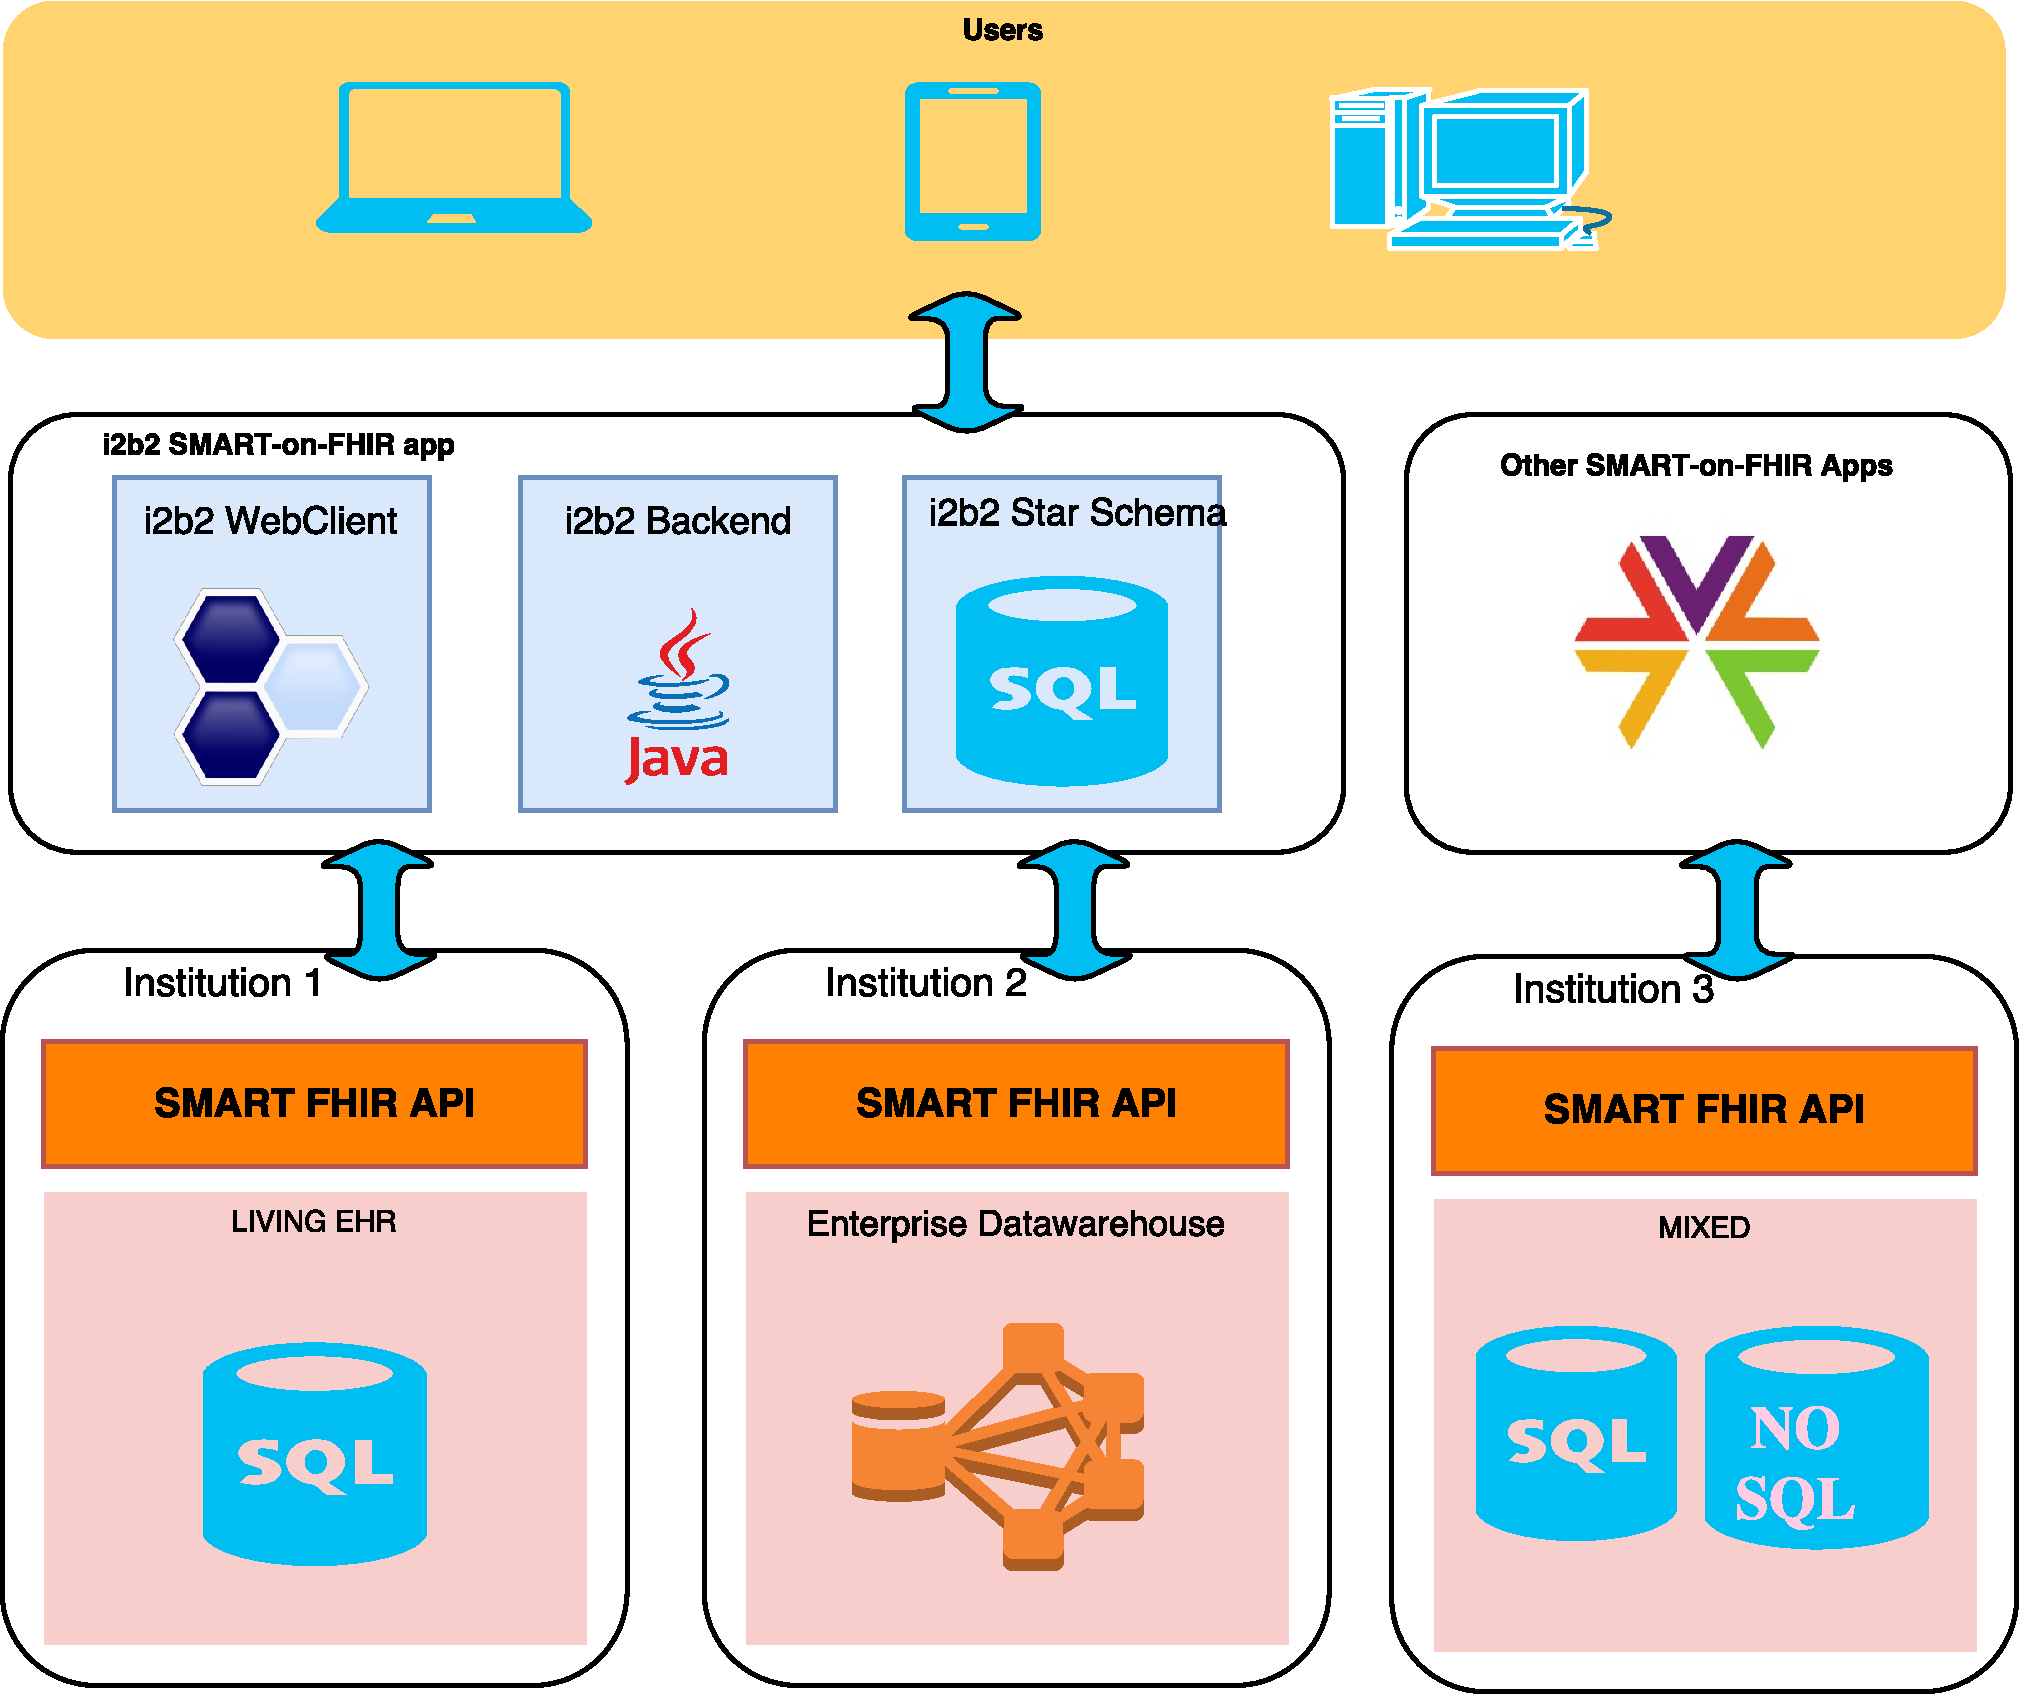
\includegraphics[scale=.45]{overall.pdf}
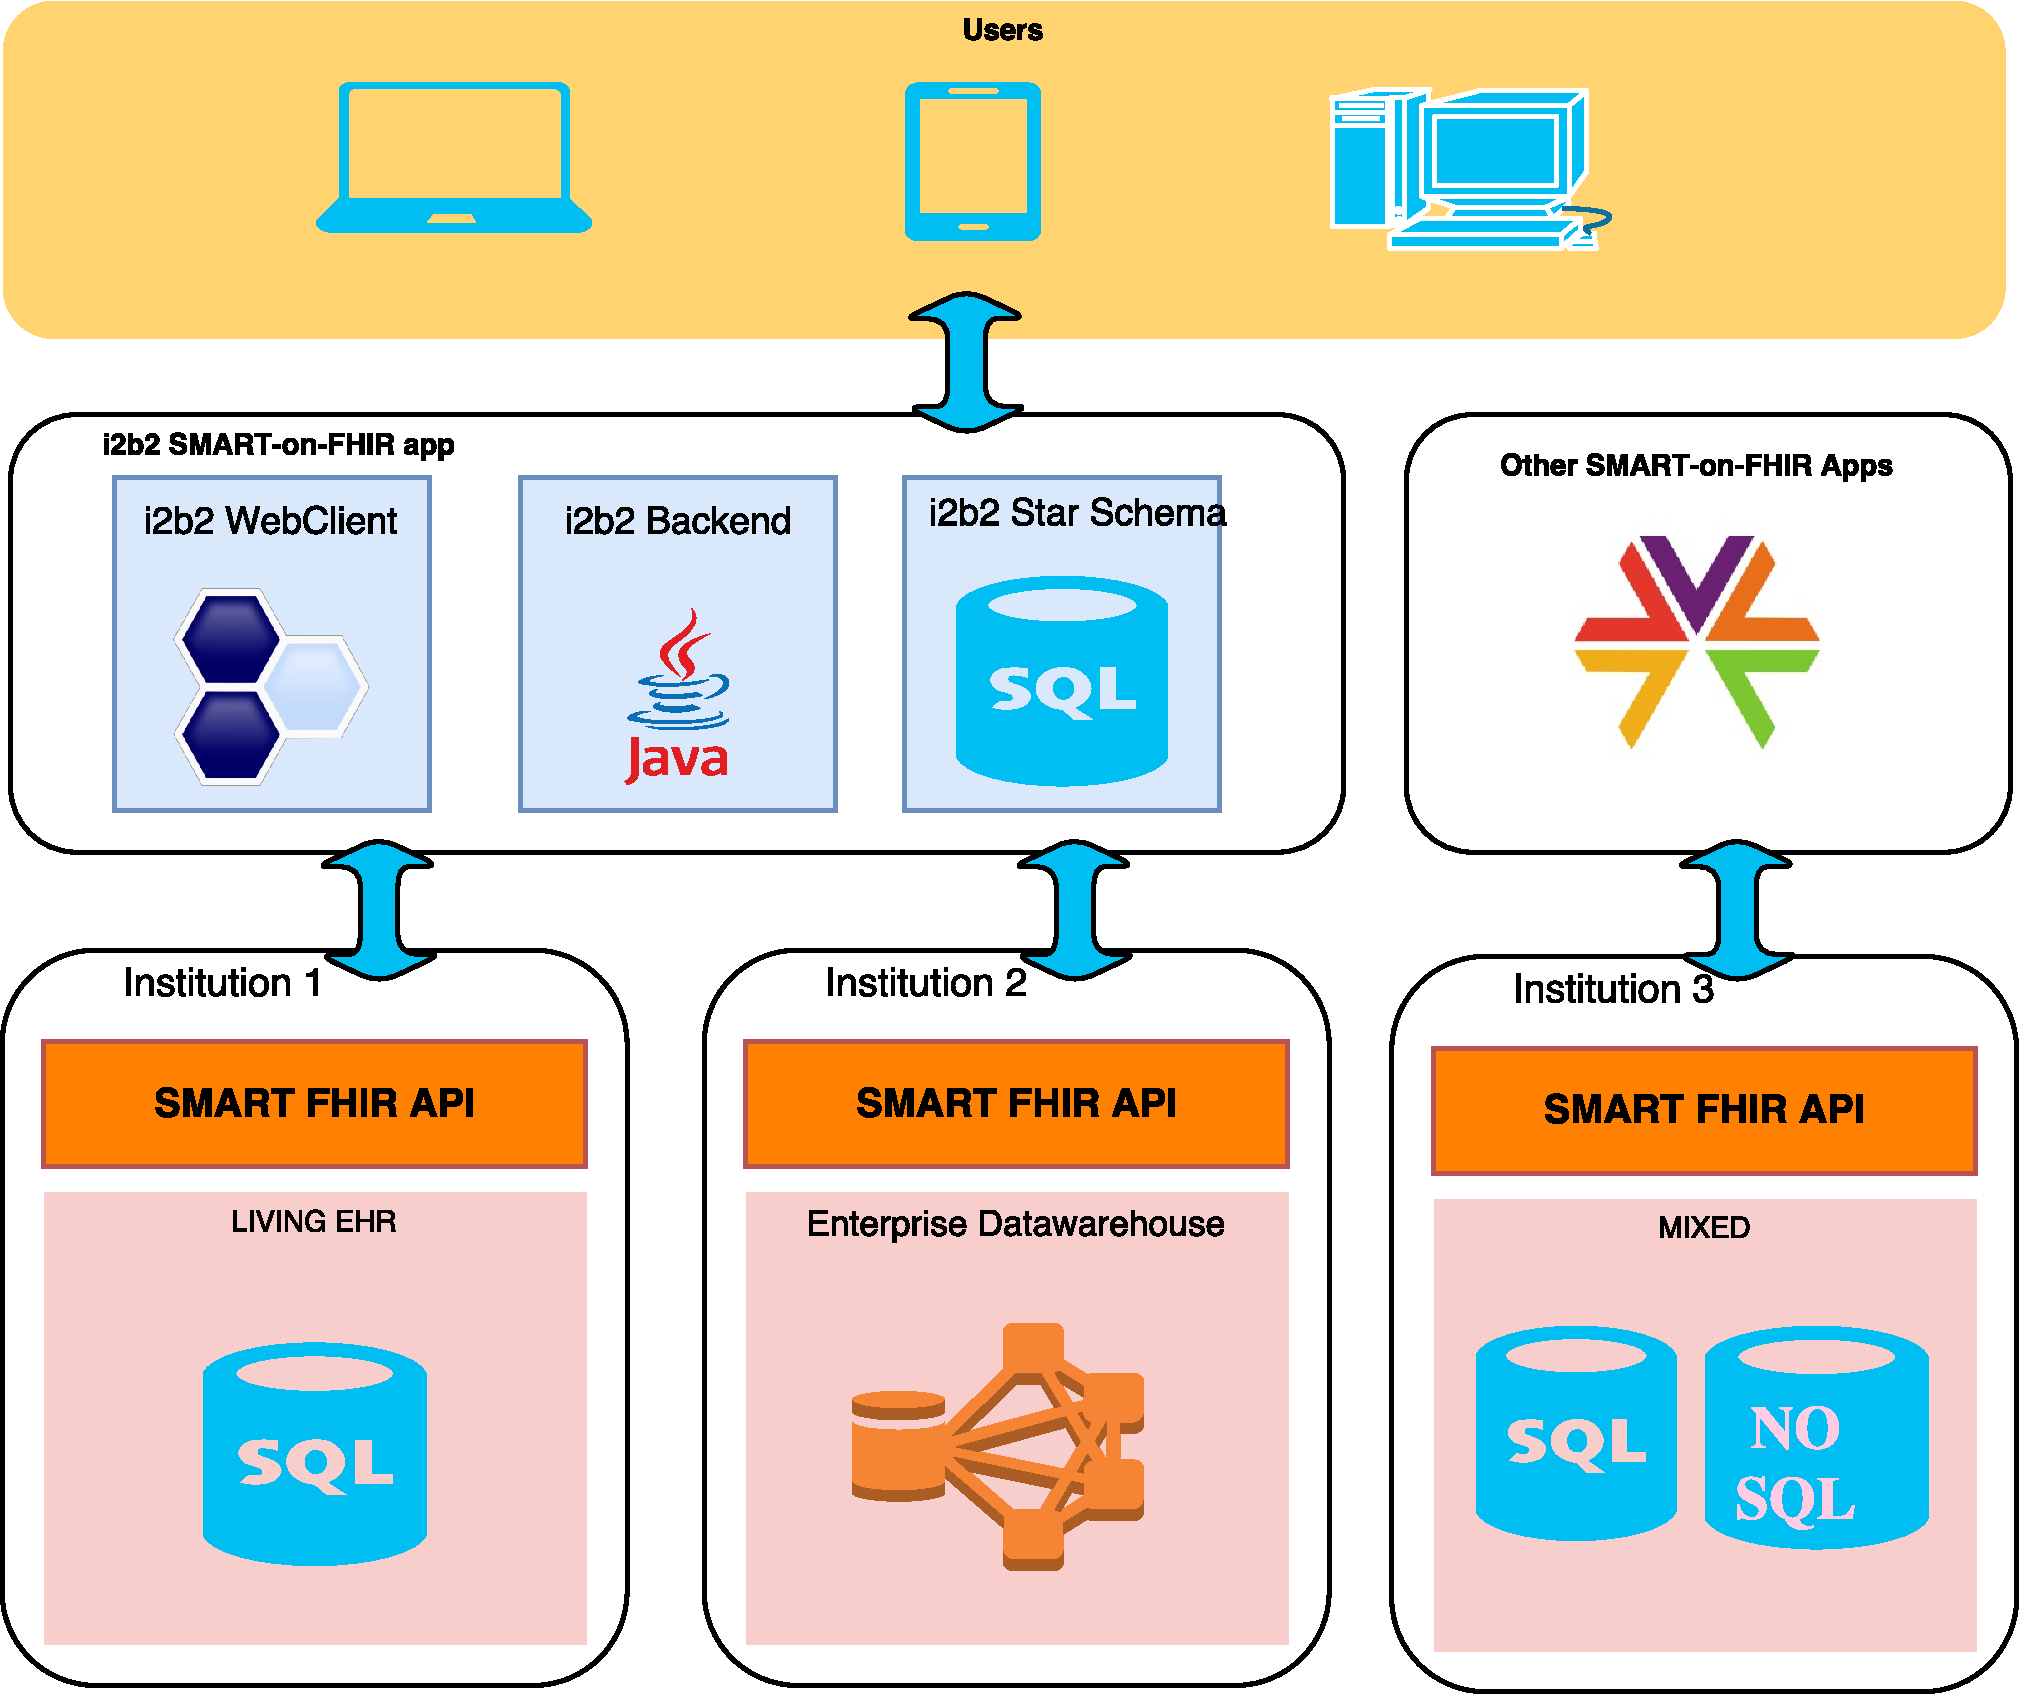
\includegraphics[width=.8\linewidth]{overall.pdf}
	\caption{Overall Diagram}
\label{overall}
\end{figure}

To meet our objectives, the existing i2b2 traditional query search module (i2b2crc) code source is extended to meet the SMART-on-FHIR API specifications and the FHIR search specifications. Figure~\ref{overall} shows the overall architecture and how the three-tier i2b2 application integrates with three remote institutions. The figure shows how an i2b2 application gives access to users in a SMART-on-FHIR application modality. In this context, users log-in to any SMART application or EHR system just once, and get access to a set of specialized applications, such as i2b2. The architecture allows queries to be combined over multiple endpoints: zero to one i2b2 star schema and/or zero to many SMART-on-FHIR APIs.

\begin{figure}[h]
\centering
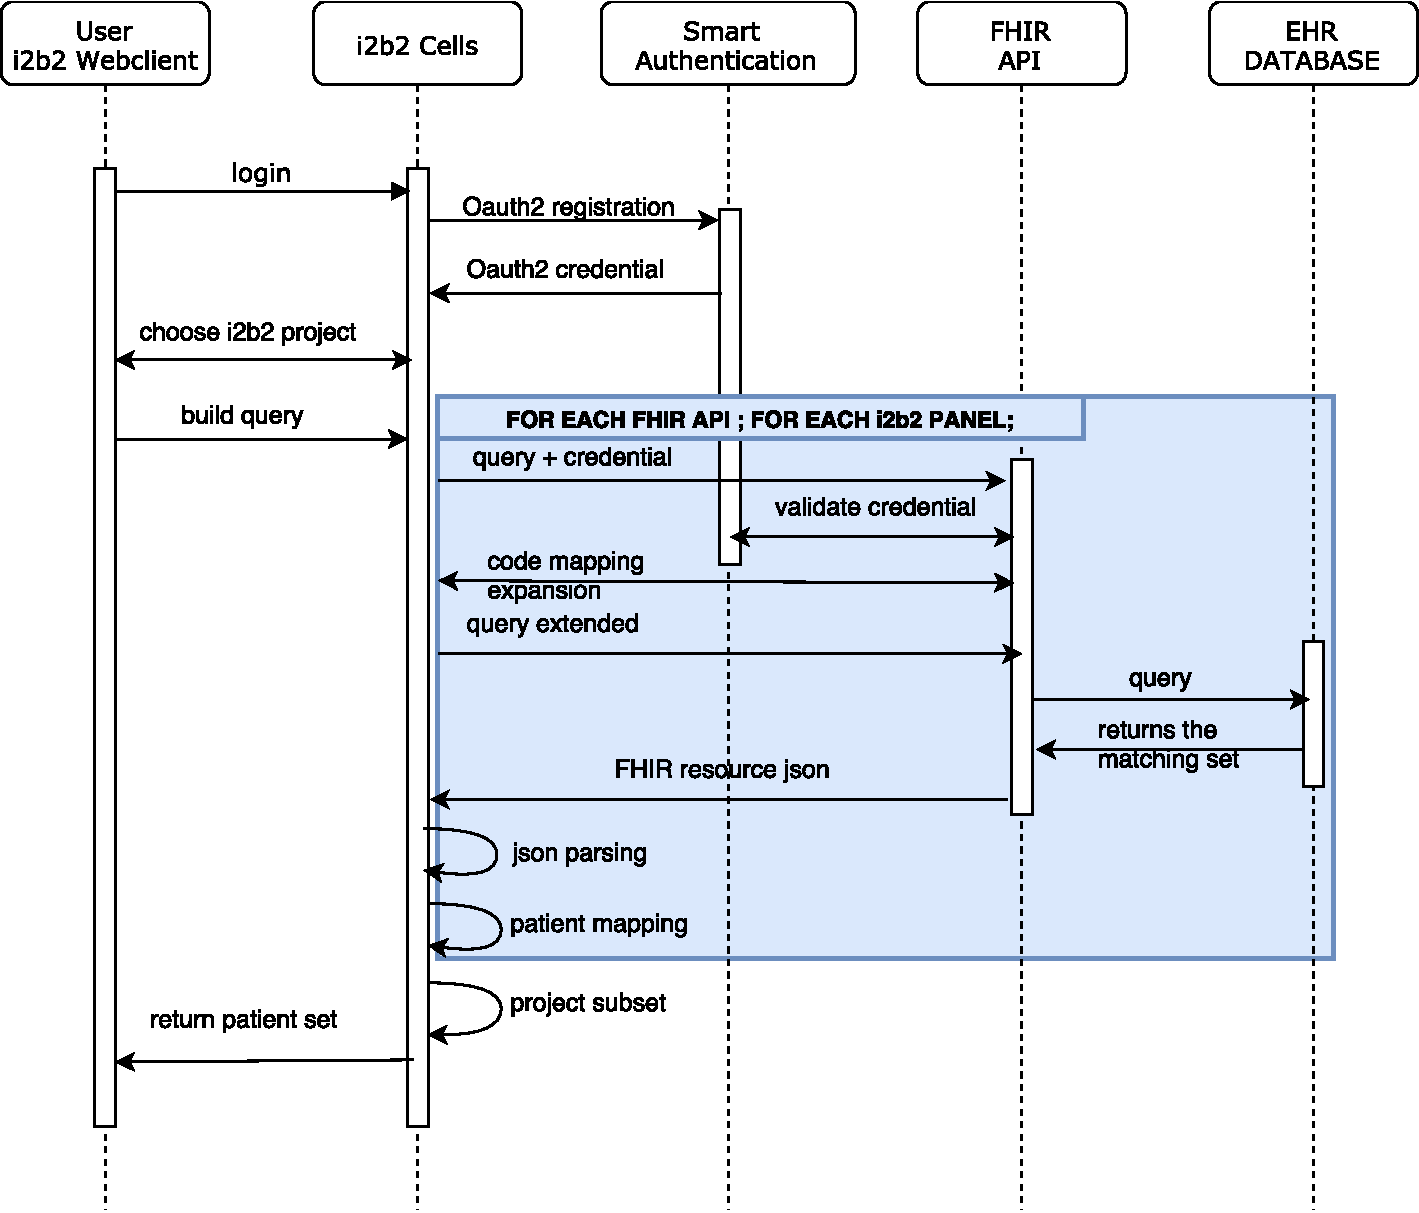
\includegraphics[scale=.6]{sequence_diagram.pdf}
\caption{UML Sequence Diagram}
\label{seq}
\end{figure}

%\remNico{Est-ce plus clair pour toi Xavier ?}
Figure~\ref{seq} is a detailed UML sequence diagram. The scenario describes a user who runs a query over an i2b2 instance containing both data in its star schema and data present in multiple remote FHIR-API endpoints. The orange arrows represent the specific new implementation carried out in this work. The user first logs into the system with his or her login credentials, which are verified by the i2b2 project management cell (i2b2pm). The i2b2pm lets the user choose within a i2b2 project list according a set of defined roles. After building and running a multiple panel query across different medical domains, the user gets back a patient cohort set by picking concepts from the i2b2 ontology. Some domains are linked to the FHIR endpoints, others are linked to the local star schema. At first, the i2b2crc conducts a patient-set lookup in its local database. Then, for the FHIR-based concepts, the system loops over the following steps against the SMART-on-FHIR API. The i2b2pm first get its Oauth2 authentication credentials because it is known as a trusted application within the SMART-Auth layer. The i2b2crc new FHIR query builder then produces the HTTP query according to the FHIR-search specifications and makes an HTTP call to the FHIR-API. This query is extended with coding synonyms defined in the FHIR ConceptMap resources (terminology server part). The resulting query is then translated by the FHIR layer in the local database query dialect to fetch the results. The result is transformed into a FHIR json bundle only containing the information needed (patient\_ids in this case). A parsing step extracts the patient\_ids. They are then mapped to a unique i2b2 identifier and pushed into a CRC temporary table that integrates all the results. Once looping is done, the i2b2crc applies a new patients security step to only keep those available for the i2b2 project selected by the user. The patient cohort set is finally returned to the user.
% * <tpollard@mit.edu> 14:51:16 28 Sep 2017 UTC-0400:
% After the sentence that says "Then, for the FHIR-based concepts, the system loops the following steps against the SMART-on-FHIR API." it should be clear that the items are a list. e.g. perhaps they should have bullet points or numbers.
% ^ <niparisco@gmail.com> 21:02:12 28 Sep 2017 UTC+0200:
% thanks, may add list if I get place. page number limited to 10
% * <tpollard@mit.edu> 14:47:23 28 Sep 2017 UTC-0400:
% UML not already defined in the document? If not, define here.
% ^ <niparisco@gmail.com> 21:01:38 28 Sep 2017 UTC+0200:
% done. Latex chooses the place itself anyway


\begin{table}[h]
\centering
	\begin{tabular}{|p{6cm}|p{10cm}|}
  \hline
    \textbf{HTTP request}    & \textbf{Description}  \\ \hline
		GET $<$FHIR-API$>$/$<$Resource$>$\newline?\_elements=$<$elements$>$\&code=$<$codes$>$\newline\&date=gt$<$date\_inf$>$\&date=lt$<$date\_sup$>$\newline\&$<$custom\_filter$>$  & Retrieves chosen $<$elements$>$ from resources optionally matching a date range or/and a list of $<$codes$>$  or/and a $<$custom\_filter$>$     \\ \hline
	 GET $<$FHIR-API$>$/ConceptMap\newline?target-code=$<$codes$>$\newline\&target-system:in=$<$code-system$>$  & Retrieves all codes that are mapped to $<$codes$>$ \& $<$code-system$>$   \\ \hline
  \end{tabular}
\caption{Index of HTTP request templates}
	\label{tab2}
\end{table}

\begin{table}[h]
\centering
	\begin{tabular}{|p{2cm}|p{6cm}|p{5cm}|}
  \hline
		\textbf{ontology table columns}    & \textbf{Description} & \textbf{Example} \\ \hline
		c\_basecode  &  FHIR code\_system / code pipe separated  & FHIR:http://loinc.com$|$1234-5  \\ \hline
		c\_tablename &  Resource / Profile pipe separated  & Observation$|$ObservationAphp  \\ \hline
		c\_metadataxml  &  An xml describing datatype (numeric, free text or enumerated) and measure units  & cf: i2b2 documentation   \\ \hline
		c\_dimcode &  an optionnal additional filter  & active=true\&status=final  \\ \hline
  \end{tabular}
\caption{i2b2 ontology adapted for FHIR}
	\label{tab1}
\end{table}

\begin{figure}

\begin{lstlisting}[language=yaml, basicstyle=\small]
version: dstu3
Patient:
    patientUriPath: $.resource.id
    patientUriField: id
Observation:
  - patientUriPath: $.resource.subject.reference,
  - encounterUriPath: $.resource.context.reference
  - instanceUriPath: $.resource.id
  - datePath: $.resource.effectiveDateTime
  - patientUriField: subject
  - encounterUriField: context
  - instanceUriField: id
  - dateField: effective
[...]
\end{lstlisting}

  \caption{i2b2-FHIR YAML configuration file sample}
	\label{conf1}
\end{figure}
\textit{FHIR-search:} FHIR search specifications\cite{FHIR} describe how to communicate with a FHIR-API to get back a set of resources matching an HTTP query criteria. The present work exploits only the possibility to fetch one type of resource per query. This is sufficient because the traditional i2b2crc allows combining multiple filter predicates by processing each one separately and then uses a deliberation step based on temporary tables. The new i2b2crc query builder replaces the SQL queries acting over the star schema to fetch record identifiers (ID) with HTTP calls to a FHIR-API. The later is then translated into the database system behind. The HTTP calls enabled in this design are presented in Table \ref{tab2}. The first row is the general template used, and is compared here with the SQL syntax (SELECT, FROM, WHERE):
\begin{description}
	\item[SELECT:] The $<$elements$>$ pattern lists the resource elements that are returned by the FHIR-API. Depending on the user choise, patient ID, encounter ID, instance ID or date are retrieved, to respectively provide i2b2 ``same patient'', ``same encounter'', ``same instance'', or ``temporal queries'' features. The way the i2b2crc retrieves those information from a given resource is described into the i2b2 FHIR config YAML file (see Figure~\ref{conf1}).
	\item[FROM:] The $<$Resource$>$ pattern is supposed to be replaced by any existing FHIR standard resource, or any profiled resource (modification of the standard to meet the local institutions constraints). In order to let the user point to the right FHIR resource, the i2b2 traditional ontology table has been reused and populated with the needed information. Table~\ref{tab1} describes how to store the information into the ``c\_tablename'' column.
	\item [WHERE:] Both patterns $<$date\_inf$>$ and $<$date\_sup$>$ allow filtering the data based on the date range defined by the user at run time. The $<$custom\_filter$>$ allows to combine a predefined pattern, such as data status, or a user-defined constraint by value query when enabled by filling the ``c\_metadataxml'' column. The $<$codes$>$ pattern can optionally contain a list of coding (e.g: SNOMED, LOINC\ldots) by populating the i2b2 ontology ``c\_basecode'' column.
\end{description}
\textit{FHIR-mapping:} The second row of Table \ref{tab2} describes the HTTP query template to enable the terminology mapping. It is then possible to the i2b2crc to use this functionality to fetch semantical synonyms that are described into the FHIR-Terminology server. As part of the ConceptMap\cite{FHIR} resource, FHIR links a source code to a target with a set of semantic ``equivalences" such as ``equivalent" or ``narrower" that characterize the way they relate to each other. The program fetches each mapping pairs and only keep the ``wider", ``subsumes", ``equal", and ``equivalent" semantic equivalence sources. The i2b2-FHIR code expansion exploits this mechanism to query over distinct code systems.

%- sequence diagram (user, i2b2, i2b2 database, smart, EMR database)
%- Example of http queries produced by i2b2-fhir-search
%- Optimisation, ask only for elements needed by i2b2


\textit{Outcome measurement:} In order to test the FHIR DSTU3 resources compatibility coverage, the HAPI FHIR\cite{HAPI} test server has been used as an endpoint since it contains useful demo datasets with fictitious patient data. The benchmark comparing traditional i2b2 and FHIR-i2b2 was carried out with the same i2b2 ``observation\_fact'' table containing 140 million records in a postgreSQL 9.6 instance. The first is based on a 1.7 i2b2 instance. The FHIR-i2b2 has been set up by implementing HAPI-FHIR server on top of the observation\_fact table into an Apache Tomcat 9 webserver, and accessed via the FHIR-i2b2 prototype. The FHIR-i2b2 big-data benchmark has been set up by implementing HAPI-FHIR server on top the ``chartevents'' MIMIC-III\cite{Johnson:SD2016} table multiplied by 15, and stored in an Apache HIVE2 table distributed over a 5-computer cluster in the Optimized Row Columnar (ORC) format distributed over HDFS. All softwares used: i2b2, HAPI-FHIR, postgreSQL and Apache Hive are open-source licensed.

\section*{Results}
% Key findings

\begin{figure}[h]
\centering
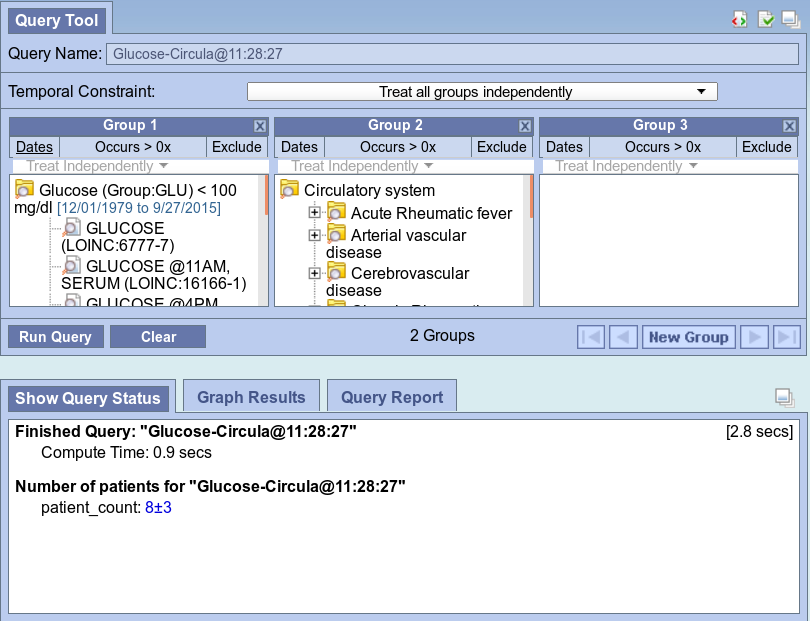
\includegraphics[scale=.4]{demo.png}
	\caption{i2b2-FHIR online demo screen-shot}
\label{fig3}
\end{figure}
\begin{figure}[h]
\centering
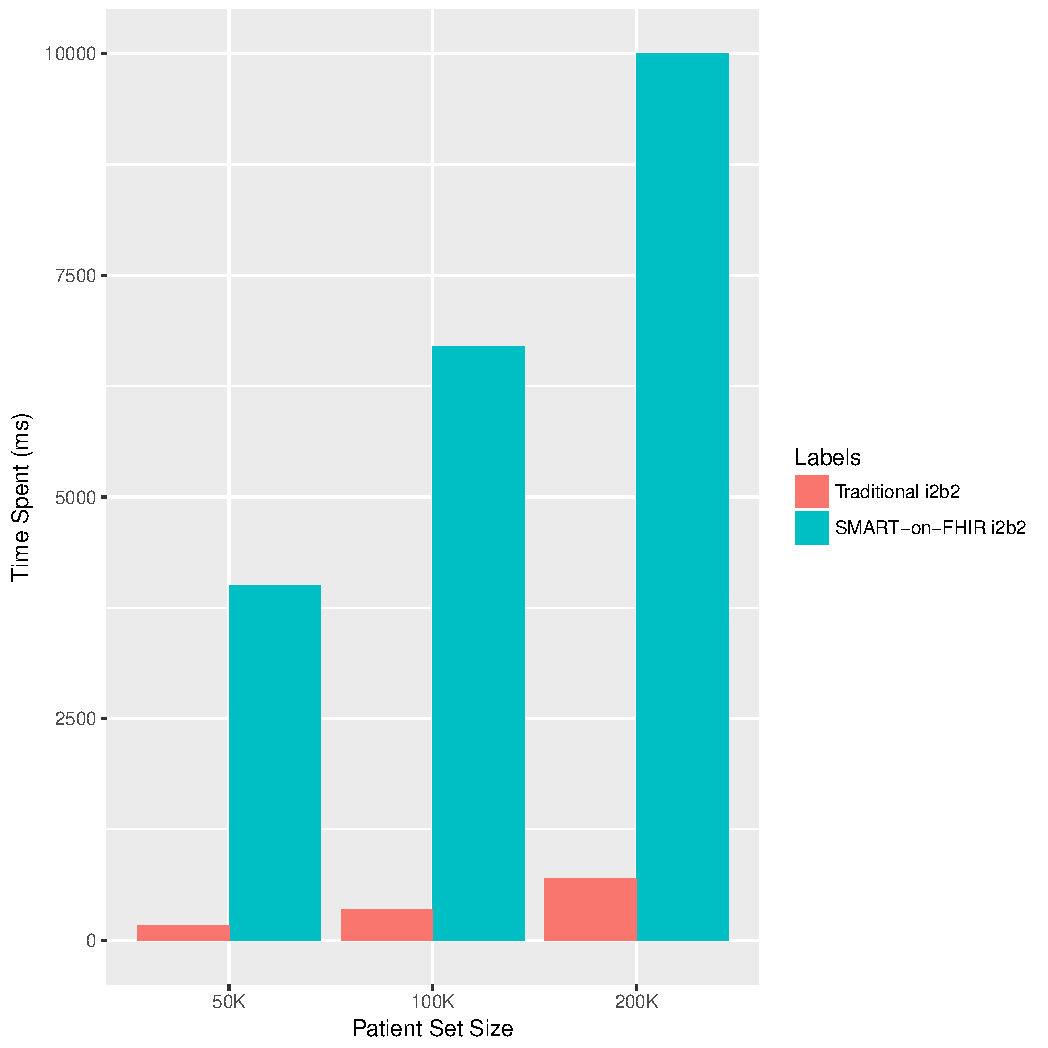
\includegraphics[scale=.6]{graph2.pdf}
	\caption{Traditional versus i2b2-FHIR performances comparison (on a 150M postgreSQL table)}
\label{fig1}
\end{figure}

\begin{figure}[h]
\centering
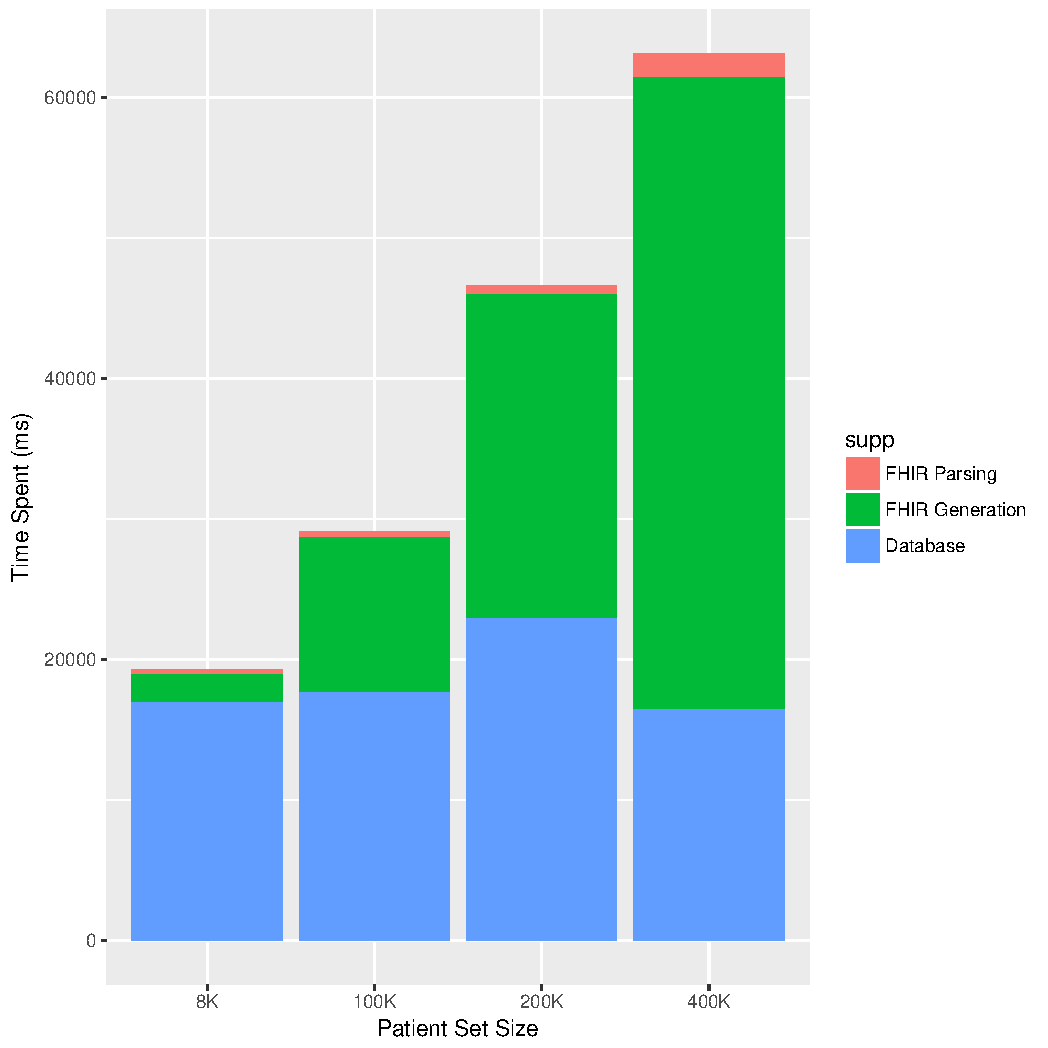
\includegraphics[scale=.6]{graph1.pdf}
	\caption{i2b2-FHIR performances (on a 5B Hive table)}
\label{fig2}
\end{figure}
\textit{Implementation Status: } The design presented below is implemented at 70\%. To date, the new i2b2crc query builder is able to query on both star schema and one remote FHIR endpoint simultaneously. Logical relations between selection criteria represented as multiple i2b2 webclient panels are also possible. The constitution of a ``patient\_set'' can be constrained by dates, values and measurement units and by one or multiple codes. The code expansion based on FHIR terminology mapping is also implemented. A living demo is deployed\cite{i2b2-fhir-demo} and a screen-shot presented in Figure \ref{fig3}. The first panel 1 query searched into HAPI FHIR test server for patients with LOINC glucose codes having value lower than 100ml/dl in a year range from 1979 to 2015 and is mixed with the second panel searching for patients having a diagnosis related to circulatory system within the star schema. The resulting ``patient\_set'' is about eight patients.

\textit{Performance:} The performance of i2b2-FHIR has been benchmarked (Figure~\ref{fig1}) versus a traditional i2b2 instance based on the star schema with the same amount of data, and configuration (140 million records). The different patient set size corresponds to different criteria selection. The histogram shows traditional i2b2 is 20 times faster than the i2b2-FHIR version. The difference can be explained by the additional steps involved: the fetched result-set is transformed into a json bundle, sent over the network and then parsed. The performance factor tends to decrease with the number of patients matched. The second benchmark (Figure~\ref{fig2}) experienced connecting to an apache HIVE table on a big-data platform containing 5 billion actual physiological patient data. The results show that the time spent is under the minute and compatible with i2b2 promises. Moreover, the bar-plots show that the major bottleneck is the FHIR json Generation step. Such quantities of data have never been described to be handled by i2b2 before, since here we approach traditional RDBMS volume limitations. While the traditional i2b2 outperforms the FHIR based i2b2 on modest datasets, the latter opens new perspectives by enabling connections with specialized and optimized database systems.


\textit{i2b2 feature coverage: }i2b2 querying feature covers filtering patients facts by code, values, dates, thought patient history, within an encounter temporal window or even a free sequence of events. By adding new temporal table mechanisms, the present work allows all of those features. Then it does not limit the existing set of functionalities. The i2b2-FHIR configuration file Figure \ref{conf1} contains information about the FHIR-API instance, such its version, and how the resources are implemented. Depending on the kind of cohort set, the user want to extract, patient ID, encounter ID, instance ID or dates are retreived from the FHIR-API thanks to a jsonPATH description. This then allows population of the CRC temporary tables. This is how i2b2 deliberation mechanisms can be populated, and the set built. Moreover the i2b2-FHIR implementation keeps backwards compatibility and does not impose FHIR-API usage for implementers that would not require it.

\textit{Security:}A security layer has been proposed and implemented into the existing i2b2crc. A new i2b2 table allows to define witch patient are part of witch i2b2 project. This security layer is important because it allows with one endpoint containing all patients records, to create multiple projects with subset allowing multiple views on the dataset. In terms of performances, the table might be vertically partitioned and spitted by project, in order to get stable performances while number of project is increasing. This mechanism is both compatible with traditional i2b2 and i2b2-FHIR and has been deployed in production at AP-HP hospital and handle more than distinct 200 projects. The Oauth2 security layer has not yet been implemented. The implementation will inspire from project\cite{Wagholikar_2016,Pfiffner__2016} that recently succeed in.

\textit{Extensibility:} The FHIR access layer has been tested over the HAPI FHIR test server for all resources at least referring to a patient (68 resources), and does have a complete resource coverage. To date, the query builder is compatible with the current FHIR DSTU3 version. In the future, it will maintain compatibility with each FHIR releases, and also backward compatibilities. The FHIR version of each endpoint is setup in the configuration file (Figure \ref{conf1}). The query builder handles the FHIR extensibility, local profiled resources or even local new resources. Moreover, the design allows to filter based on FHIR extensions, thanks to the i2b2 ontology table ''c\_dimcode'' with its custom filters. The results let conclude the design is flexible enough to query multiple centers with different FHIR implementations at the same time.

\textit{Interoperability: }FHIR-ConceptMap expansion has been implemented. A set of test mapping have been produced and populated into HAPI-FHIR to make the proof of concept. The HTTP query described into Table \ref{tab2} (row 2)  allows to fetch the equivalent codes. While their is some field of improvement, the results open area for massive and collaborative concept mapping, with a terminology server FHIR compatible. Interoperability is also derived from the FHIR standard resource definition. However, the ability to derive from them and build Profiled Resources is handled by the i2b2-FHIR YAML configuration flexibility together with the i2b2 ontology table, as they are designed to be adapted.

\section*{Discussion}

FHIR abstraction allows designing mixed architecture based on living EHR and big-data storage to leverage massive and unstructured clinical data. One can choose the best technology depending on the expected usage and local specificity of the data. The flexible design allows implementers to define their own i2b2 ontologies. Finally, an i2b2 federation over FHIR is able to bridge multiple FHIR implementations at the same time. The querying benchmarks showed that performance was not an issue. Moreover, by leveraging access to big-data technologies, this opens a new-area of specific solution to manage the diversity, variety and volume of healthcare data such Genomics, Imaging, Physiological Monitoring. The abstraction provided by the FHIR layer allows plugging new text specific technologies based on Apache Lucene, such SOLR \& Elastic search. This will allow clinicians to mine text as simply as a modern search engine does. The interoperability gain from the FHIR interface let envisage to query multiple center the same way on real-time data. The security was enforced and allows multiple sub projects to access to subsets of the whole patients database. This addresses the patient research opposition and allows studies to only access to data needed.
% * <tpollard@mit.edu> 17:20:32 28 Sep 2017 UTC-0400:
% This sentence needs checking - "...possible. - free text search"
% ^ <niparisco@gmail.com> 23:25:30 28 Sep 2017 UTC+0200:
% true, done

Several modules have been implemented, some aspects of the design have only been tested as separate modules. The roadmap provides for the development of multiple SMART-on-FHIR endpoints access, Oauth2 implementation and performances improvements. Once satisfied with the results, the system should be available in next releases of core i2b2. Specific exploration around specialized databases (temporal-series, text-mining, distributed, graph databases) will result to better handling variety of big-data, such genomic\cite{Alterovitz_2015}, textual notes, DICOM imaging, physiological waveforms or exposomic.

While all resources containing patient reference where tested, there is a need to propose a general mapping between traditional i2b2 objects (patient, visit, provider, observation) and FHIR specific resources (Organization, HealthcareService, Patient, EpisodeOfCare, Condition, Procedure, Medication, MedicationRequest, Observation, DiagnosticReport, ClinicalImpression\ldots). A general algorithm to translate FHIR terminologies into i2b2 ontology will also be investigated, and result as a complementary software.


\section*{Conclusion}

By bridging current modern solution in the field of medical data, this work paves the ways of improvements to addresses current Learning Health Systems challenges.
The challenges of \textit{data federation}, \textit{data interoperability}, \textit{data freshness} and \textit{data security} can benefit from both i2b2 experiences and 
FHIR simplifications.
The challenges of \textit{data volume} and \textit{data variety} of medical datasets are indirectly addressed by the FHIR-API abstraction that makes possible the use of 
powerful and dedicated technology.

In the end, while a tool that is able to bridge international institutions together is likely to emerge, the concept mapping between such many institutions remains to be done. Since all are based on different languages, different granularity and different concept and practices, this remains a challenge to be addressed. While ontology matching is an old research area, it is an area that still presents significant challenges to overcome.

%The main contribution of the work is to pave the way for cohort-generation process by leveraging standard access, with interoperable terminology systems and state of the art security methods. The hospital centers international effort to converge to FHIR data exchange layer[ref] will ease the data-federation to query center without dedicated datawareouhsing staff. The main advantage over other approach to federate clinical repository such SHRINE, or Insite, is it benefits from FHIR ConceptMap and FHIR search that are already in place for other uses case in the institutions.
%The secondary contribution of the work is to allow implementers to use their own technology, and allow i2b2 instance to benefits from the fast past and future improvements on big-data technologies.

%Cross-border networking coordination and new technologies for data integration facilitates interoperability among research networks. Clinical research is on the threshold of a new era in which electronic health records (EHRs) are gaining an important novel supporting role. i2b2 has been extended to allow multicentric querying within research networks.  This paper proposed a new approach for linking i2b2 to EHRs.

\makeatletter
\renewcommand{\@biblabel}[1]{\hfill #1.}
\makeatother

\bibliographystyle{unsrt}
\bibliography{biblio}
%\begin{thebibliography}{1}



%
% BIBLIO MOVED TO biblio.bib
%




%\end{thebibliography}
\end{document}
